\documentclass[10pt]{beamer}
\usetheme[background=light,block=fill,progressbar=foot]{metropolis}
%\usepackage[UTF8]{ctex}
\usepackage{graphicx}
\usepackage{caption}
\usepackage{bm}
%\usepackage{coloremoji}
\newcommand{\supercite}[1]{\textsuperscript{\textsuperscript{\cite{#1}}}}
\newcommand{\emoji}[1]{\text{\raisebox{-0.2em}{\includegraphics[height=1em]{emojis/#1.png}}}}
%\usefonttheme[onlymath]{serif}

\begin{document}
	\title{Deep Learning Book}
	\subtitle{Chapter 6 \\ Deep Feedforward Networks}
	\author{Botian Shi \\ botianshi@bit.edu.cn}
	\date{\today}

	\begin{frame}[plain]
		\titlepage
	\end{frame}

	\begin{frame}
		You can download the \LaTeX\, source code of this file from \href{https://github.com/friskit-china/DLBookSlides}{\underline{Here}}.
	\end{frame}
	
	\begin{frame}{Feedforward Networks}
		
		\begin{itemize}
			\item A type of neural network
				\begin{itemize}
					\item \emph{Deep feedforward network}
					\item \emph{feedforward neural network}
					\item \emph{multilayer perceptron (MLP)}
				\end{itemize}
			\item For a classifier, $y = f^{\,*}(\bm{x})$ maps an input $\bm{x}$ to category $\bm{y}$
			\item Defines a mapping:
					\begin{center}
						$\bm{y}=f(\bm{x};\bm{\theta})$
					\end{center}
			\item Learns the best approximation of $f^{\,*}$ with parameter $\bm{\theta}$
			\item Feedforward only, no feedback connections.
			\item The basis of many applications.
		\end{itemize}
	\end{frame}

	\begin{frame}{Feedforward networks are ...}
		\begin{enumerate}
			\item Extreme important.
			\item Stepping stone on the path to recurrent neural networks.
		\end{enumerate}
		\begin{exampleblock}{Example: convolutional neural network}
			\begin{figure}
				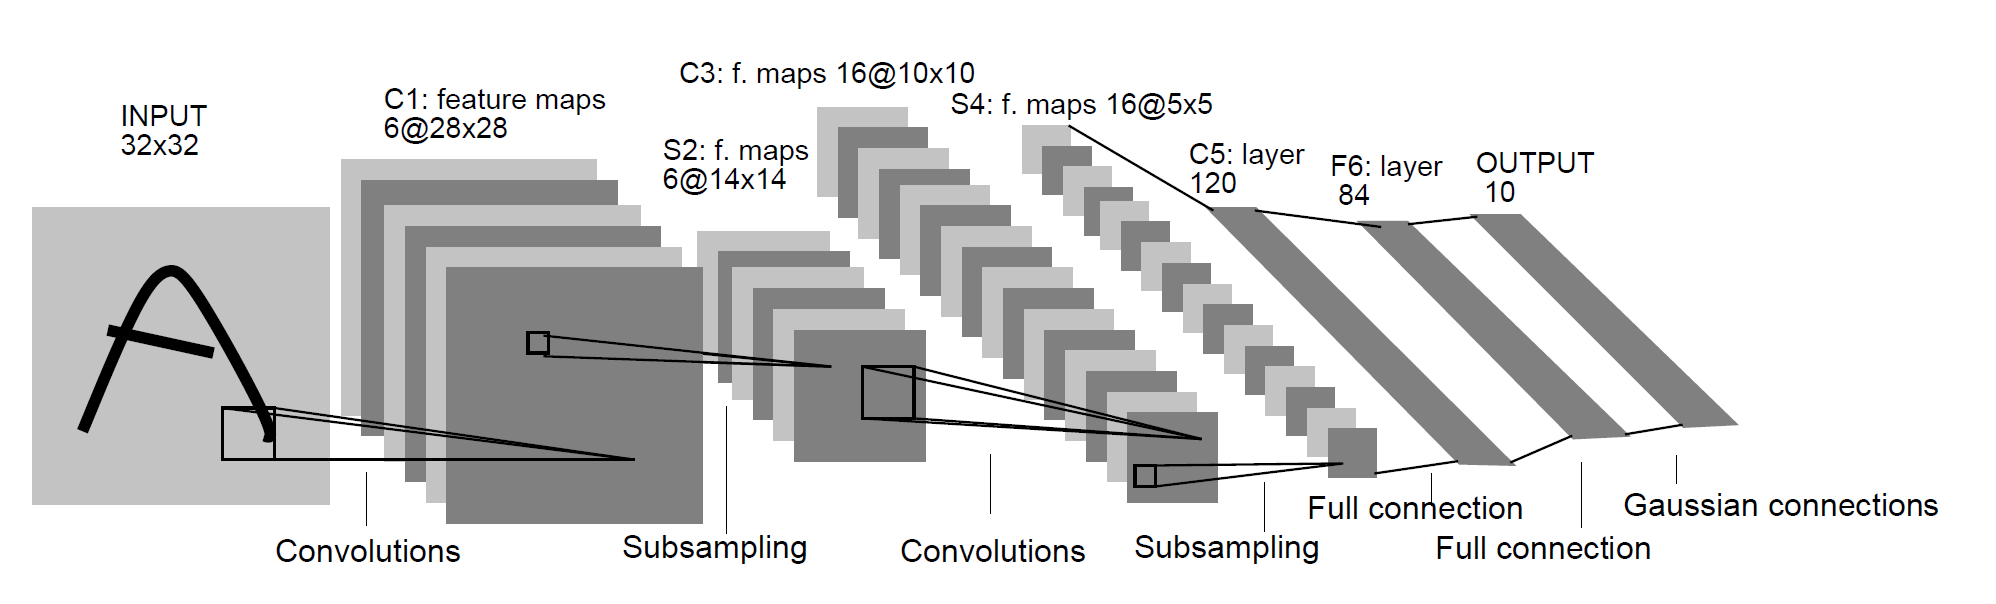
\includegraphics[width=25em]{figures/lenet-5.png}
				\caption{A type of convolutional neural network: LeNet-5\supercite{lecun1998gradient}}
			\end{figure}
		\end{exampleblock}
	\end{frame}

	\begin{frame}{Multilayer Perceptron}
		\begin{columns}[T,onlytextwidth]
			\column{0.7\textwidth}
			\begin{itemize}
				\item Why called \emph{networks}?
				\begin{itemize}
					\item Composing together many different functions.
					\item Model is associated with a DAG describing the composition.
					\begin{equation*}
					f(\bm{x}) = f^{\,(3)\,}(f^{\,(2)\,}(f^{\,(1)\,}(\bm{x})))
					\end{equation*}
					\item $f^{\,(1)\,}$ called first layer of the network
					\item $f^{\,(2)\,}$ called second layer, and so on
					\item $f^{\,(2)\,}$ called output layer
				\end{itemize}
			\end{itemize}
			\column{0.3\textwidth}
			\begin{figure}
				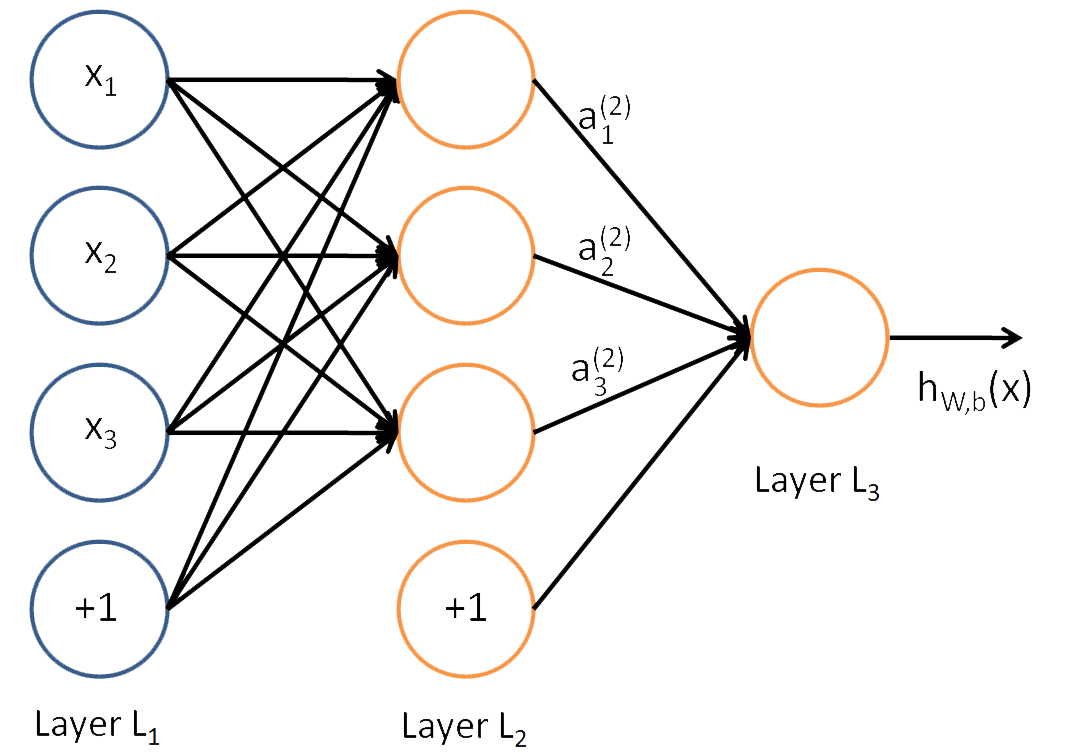
\includegraphics[width=10em]{figures/multilayer-perceptron.png}
				\caption{\\ An example of MLP  (from \href{http://ufldl.stanford.edu/wiki/index.php/File:Network331.png}{UFLDL})}
			\end{figure}
		\end{columns}
		\begin{itemize}
			\item During training, we drive $f\,(\bm{x})$ to match $f^{\,*}(\bm{x})$
			\item Each example $\bm{x}$ is accompanied by a label $y\approx f^{\,*}(\bm{x})$
			\item At each point $\bm{x}$, network must produce a value that is close to $\bm{y}$.
			\item The learning algorithm must decide how to use those layers to produce the desired output.
			\item Layers between input and output layer are called \emph{hidden layer}.
		\end{itemize}
	\end{frame}

	\begin{frame}{The \emph{NEURAL} network}
		\begin{itemize}
			\item Inspired by neuroscience.
			\begin{columns}
				\column{0.5\textwidth}
				\begin{figure}
					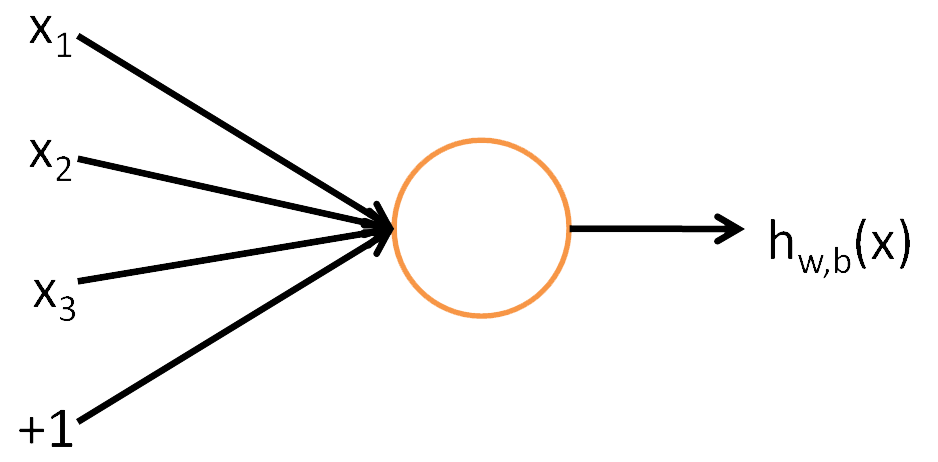
\includegraphics[height=5em]{figures/neuron.png}
					\caption{Neuron (from \href{http://deeplearning.stanford.edu/wiki/index.php/File:SingleNeuron.png}{UFLDL})}
				\end{figure}
			
				\column{0.5\textwidth}
				\begin{figure}
					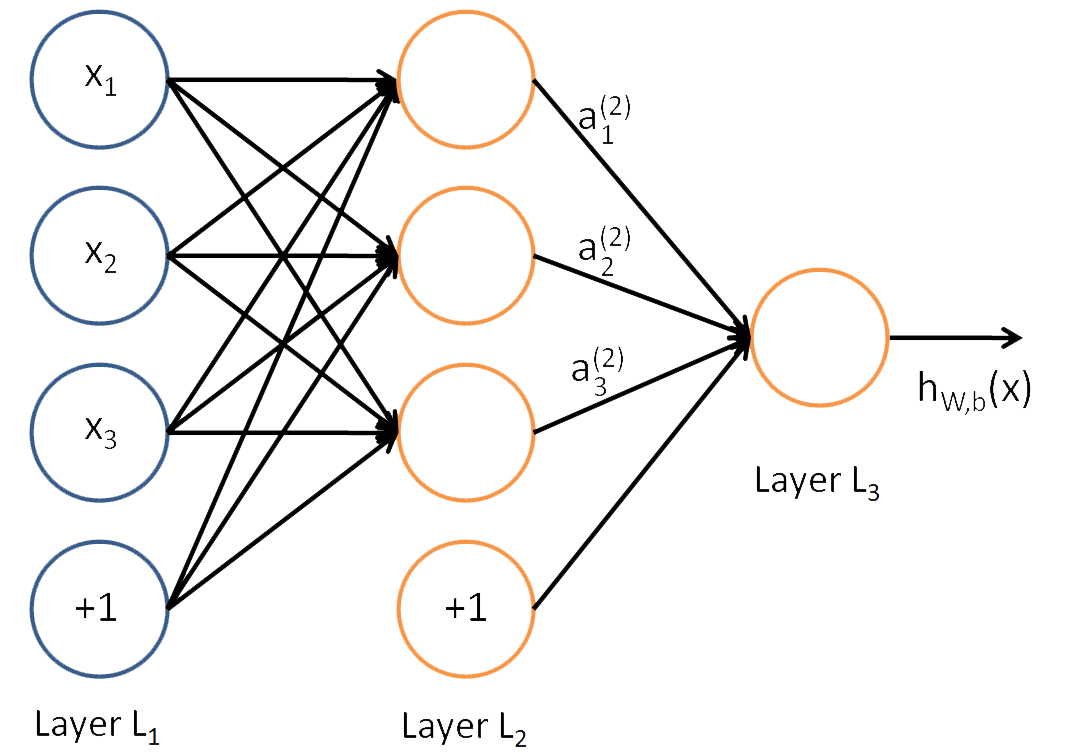
\includegraphics[height=5em]{figures/multilayer-perceptron.png}
					\caption{MLP (from \href{http://ufldl.stanford.edu/wiki/index.php/File:Network331.png}{UFLDL})}
				\end{figure}
					
			\end{columns}
			\item Each hidden layer is vector-valued. The dimensionality of these hidden layers determines the \emph{width} of the model.
			\item Each element of the vector may be interpreted as a neuron.
			\item Layer consist of many \emph{units} that act in parallel, each representing a vector-to-scalar function.
			\item Each unit resembles a neuron that receives input from many other units and computes its own activation value.
		\end{itemize}
	\end{frame}

	\begin{frame}{The \emph{NEURAL} network}
		\begin{itemize}
			\item The idea of using many layers of vector-valued representation is drawn from neuroscience.
			\item Modern neural network research $\ne$ perfectly model the brain.
			\item Feedforward networks $\approx$ function approximation machines.
			\item Inspired by brain, rather than model a brain.
		\end{itemize}
	\end{frame}
	
	\begin{frame}{Understand feedforward networks}
		\begin{itemize}
			\item Linear Models
			\begin{exampleblock}{Linear Regression}
				\vspace{-2em}
				\begin{center}
					$$h_\theta(\bm{x};\theta)=\theta ^T\bm{x}=\theta_0+\theta_1x_1+\theta_2x_2+\dots+\theta_nx_n$$	
					\vspace{-2em}
					$$\theta=\mathop{\arg\min}_{\theta}\mathrm{J}(\theta;\bm{X})=\mathop{\arg\min}_{\theta}\frac{1}{2}\sum^{m}_{i=1}(h_\theta(x^{(i)})-y^{(i)})^2$$
					\vspace{-1em}
				\end{center}
			\end{exampleblock}
			
			\begin{exampleblock}{Logistic Regression}
				\vspace{-1.5em}
				\begin{center}
					$$h_\theta(\bm{x};\theta)=g(\theta^T\bm{x})=\frac{1}{1+e^{-\theta^T\bm{x}}}$$
					\vspace{-1.5em}
					$$g(z)=\frac{1}{1+e^{-z}}$$
					\vspace{-1.5em}
				\end{center}
			\end{exampleblock}
			
			\begin{exampleblock}{General Linear Model}
				$$p(y;\eta)=b(u)\exp(\eta^TT(y)-a(\eta))$$
			\end{exampleblock}
		\end{itemize}
		
	\end{frame}
	
	\begin{frame}{Understand feedforward networks}
		\begin{itemize}
			\item Efficiently and reliable
			\item The model capacity is limited to linear functions.
			\begin{itemize}
				\item The model cannot understand the interaction between any two input variables.
			\end{itemize}
			\item To extend linear models to represent nonlinear functions of $\bm{x}$, we can apply the linear model not to $\bm{x}$ itself but to a transformed input $\phi(\bm{x})$, where $\phi$ is a \emph{nonlinear transformation}.
			\item $\phi$ provide a set of features describing $\bm{x}$, or provide a new representation fo $\bm{x}$
		\end{itemize}
	\end{frame}
	
	\begin{frame}{Understand feedforward networks}
		\begin{itemize}
			\item How to choose $\phi$?
			\begin{enumerate}
				\item Use a very generic $\phi$, e.g., infinite-dimensional $\phi$.
				\begin{itemize}
					\item High dimension $\Leftrightarrow$ enough capacity to fit the training set.
					\item High dimension $\Leftrightarrow$ poor generalization capacity.
					\item More is less: Runge phenomenon; Gibbs phenomenon 
%					\begin{figure}
%						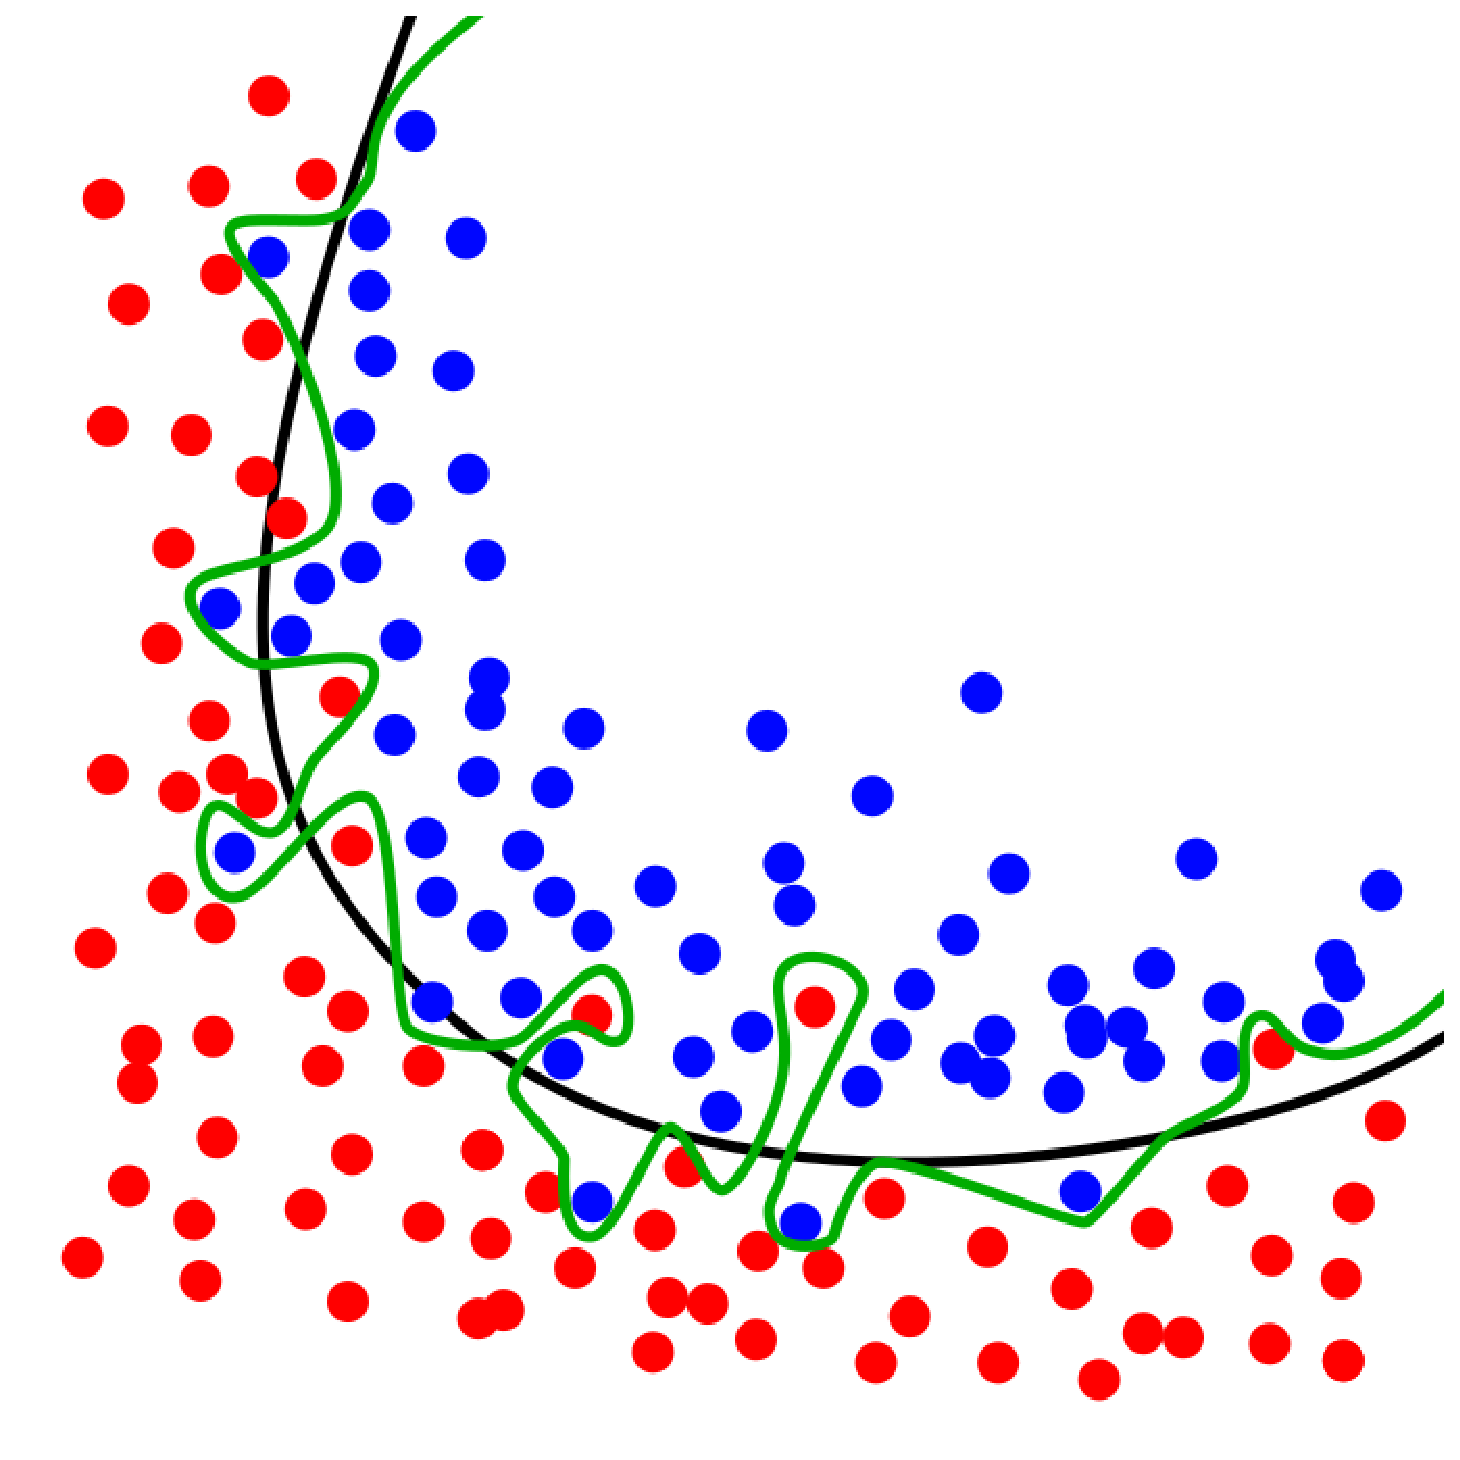
\includegraphics[height=10em]{figures/overfitting.eps}
%						\caption{Overfitting (from: \href{https://commons.wikimedia.org/wiki/File:Overfitting.svg}{Wikepedia})}
%					\end{figure}
				\end{itemize}
				\item Manually engineer $\phi$.
				\begin{itemize}
					\item Require human effort for each separate task.
					\item Need practitioners specializing in different domains.
				\end{itemize}
				\item Deep learning.
				\begin{itemize}
					\item Strategy: learn a $\phi$.
					\item $y=f(\bm{x};\bm{\theta},\bm{w})=\phi(\bm{x};\bm{\theta})^T\bm{w}$
					\item We have parameters $\theta$ to learn $\phi$ from a broad class of functions.
					\item We have parameters $\bm{w}$ to map from $\phi(\bm{x})$ to the desired output.
					\item Here in example, $\phi$ defining a hidden layer.
					\item Deep learning is not simply a \emph{deep} neural network. The $\phi$ is crucial!
				\end{itemize}
			\end{enumerate}
		\end{itemize}
	\end{frame}
	
	\begin{frame}{Understand feedforward networks}
		\begin{itemize}
			\item Why deep learning?
			\begin{enumerate}
				\item Parametrize the representation as $\phi(\bm{x};\bm{\theta})$
				\item We can use optimization algorithm to find the $\bm{\theta}$ that corresponds to a good representation.
				\item Capture the benefit of first and second approach.
				\begin{itemize}
					\item Being highly generic: using a very broad family $\phi(\bm{x};\bm{\theta})$
					\item Human practitioners can encode their knowledge by designing families $\phi(\bm{x};\bm{\theta})$.
					\item Human designer only needs to find the right general function family rather than finding precisely the right function.
				\end{itemize}
			\end{enumerate}
			\item The general principle of deep learning is to improve models by learning feature representation.
			\item Feedforward networks are the application of this principle to learning deterministic mappings from $\bm{x}$ to $\bm{y}$ that lack feedback connections.
		\end{itemize}
	\end{frame}
	
	\begin{frame}{Deploy a feedforward network}
		Training a feedforward network requires the same design decisions for linear model:
		\begin{itemize}
			\item Define the form of input and output units.
			\item Designthe architecture of the network
			\begin{enumerate}
				\item How many layers the network should contain
				\item How these networks should be connected to each other
				\item How many units should be in each layer.
			\end{enumerate}
			\item Choose activation functions for hidden layers.
			\item Define a cost function
			\item Choose an optimizer (gradient descent algorithm and its modern generalizations) to train the network.
			\item Use back-propagation algorithm to compute the gradients of complicated functions.
		\end{itemize}
	\end{frame}


	\begin{frame}[allowframebreaks]{References}
		\bibliography{Chap6}
		\bibliographystyle{abbrv}
	\end{frame}

\end{document}